\section{Čísla}

\begin{pozadavky}
\begin{pitemize}
\item Vlastnosti přirozených, celých, racionálních, reálných a komplexních čísel
\item Posloupnosti a limity
\item Cauchyovské posloupnosti
\end{pitemize}
\end{pozadavky}

\subsection{Reálná čísla}
Množinou všech reálných čísel (značíme ji $\mathbb{R}$) budeme rozumět množinu, na níž je definováno sčítání (značíme $x+y$), násobení (značíme $x\cdot y$) a uspořádání (značíme $x \le y$), která spňují tyto axiomy:

\begin{penumerate}
	\item (Algebraické operace)
	\begin{penumerate}
		\item $\forall x,y,z \in \mathbb{R} : x+(y+z) = (x+y)+z \hfill\textit{(asociativní zákon pro sčítání)}$
		\item $\forall x,y \in \mathbb{R} : x+y = y+x \hfill\textit{(komutativní zákon pro sčítání)}$
		\item v $\mathbb{R}$ existuje nulový prvek (značíme ho 0) tak, že $\forall x \in \mathbb{R}: x+0 = x$
		\item pro každý $x \in \mathbb{R}$ existuje opačný prvek (značíme ho $-x$) tak, že $x+(-x)=0$
		\item $\forall x,y,z \in \mathbb{R}: x\cdot (y\cdot z)=(x\cdot y)\cdot z \hfill\textit{(asociativní zákon pro násobení)}$
		\item $\forall x,y \in \mathbb{R} : x\cdot y = y\cdot x \hfill\textit{(komutativní zákon pro násobení)}$
		\item v $\mathbb{R}$ existuje jednotkový prvek (značíme ho 1) tak, že $\forall x \in \mathbb{R}: x\cdot 1=x$
		\item pro každý $x \in \mathbb{R}, x \neq 0$ existuje inverzní prvek (značíme ho $x^{-1}$) tak, že $x\cdot x^{-1}=1$
		\item $\forall x,y,z \in \mathbb{R}: (x+y)\cdot z = x\cdot z + y\cdot z \hfill\textit{(distributivní zákon)}$
	\end{penumerate}
	\item (Uspořádání)
	\begin{penumerate}
		\item $\forall x,y,z \in \mathbb{R}: ((x \le y) \wedge (y \le z)) \Rightarrow (x \le z) \hfill\textit{(tranzitivita)}$
		\item $\forall x,y \in \mathbb{R}: (((x \le y) \wedge (y \le x)) \Rightarrow (x=y) \hfill\textit{(slabá antisymetrie)}$
		\item $\forall x,y \in \mathbb{R}: (x \le y) \vee (y \le x)$
		\item $\forall x,y,z \in \mathbb{R}: (x \le y) \Rightarrow (x+z \le y+z)$
		\item $\forall x,y,z \in \mathbb{R}: (x \le y) \wedge (0 \le z) \Rightarrow (x\cdot z \le y\cdot z)$
	\end{penumerate}
	\item (Netrivialita)
	\begin{penumerate}
		\item $0 \neq 1$
	\end{penumerate}
	\item (Úplnost)
		\\\begin{definiceN}{Axiom suprema}
		Nechť $M \subset \mathbb{R}$ je neprázdná a shora omezená. Pak existuje číslo $s \in \mathbb{R}$, které má vlastnosti:
		\begin{penumerate}
			\item $\forall x \in M: x \le s$
			\item $\forall s' \in \mathbb{R}, s' < s\;\; \exists x \in M: x > s'$
		\end{penumerate}
		
		Číslo $s$ z axiomu suprema je jednoznačně určeno, značí se $\sup M$ a říká se mu \emph{supremum množiny $M$}. Supremum množiny je její nejmenší horní závora (\emph{horní závora} je každý takový prvek, pro který platí bod (a) definice suprema). Největší dolní závoru množiny $M$ (pokud existuje -- a dá se dokázat, že existuje, je-li množina zdola omezená) nazýváme \emph{infimem množiny $M$} a značíme $\inf M$.
		\end{definiceN}
\end{penumerate}

\begin{poznamka}
Relace \uv{$<$} na reálných číslech (a stejně tak na přirozených a racionálních číslech) se definuje takto: $a<b$, právě když $a\leq b$ a zároveň $a\neq b$.
\end{poznamka}

\subsection{Přirozená čísla}

\begin{definice}
	Řekneme, že množina $S \subset \mathbb{R}$ je \emph{induktivní}, jestliže platí
	\begin{pitemize}
		\item $1 \in S$
		\item $[x \in S \Rightarrow (x+1) \in S]$
	\end{pitemize}
	Množinu \emph{přirozených čísel $\mathbb{N}$} definujeme jako průnik všech induktivních podmnožin $\mathbb{R}$, tedy
	$$
		N := \bigcap \{ S; S \subset \mathbb{R}; \textit{S induktivní}\}
	$$
\end{definice}

\begin{vetaN}{Induktivnost přirozených čísel}
	Množina $\mathbb{N}$ je induktivní.
\end{vetaN}

\begin{vetaN}{Vlastnosti přirozených čísel}
	Množina $\mathbb{N}$ má nasledujúcí vlastnosti:
	\begin{penumerate}
		\item $n \in \mathbb{N} \Rightarrow n \ge 1$
		\item $n \in \mathbb{N} \backslash \{1\} \Rightarrow \exists m \in \mathbb{N}: n=m+1$
		\item $m,n \in \mathbb{N}, m < n \Rightarrow m + 1 \le n$ %před pravou stranou \exists byt nemusi -- Tuetschek
		\item každá neprázdná podmnožina $\mathbb{N}$ má nejmenší prvek
	\end{penumerate}
\end{vetaN}

\begin{vetaN}{Archimédova vlastnost reálných čísel}
	Pro každé $x \in \mathbb{R}$ existuje $n \in \mathbb{N}$ takové, že $x < n$
\end{vetaN}

\begin{vetaN}{Peanove axiómy pre zavedenie prirodzených čísel}
\begin{pitemize}
	\item Existuje číslo 0 (to neznamená, že nula je prirodzené číslo, v $\mathbb{N}$ roli tejto nuly hraje jednotka).
	\item Na množine prirodzených čísel je definovaná unárna operácia \uv{nasledovník}, označovaná S.
	\item Neexistuje žiadne prirodzené číslo, ktorého nasledovníkom je 0.
	\item Rôzne prirodzené čísla majú rôznych nasledovníkov: $a \neq b \Rightarrow S(a) \neq S(b)$ (t.j. funkcia nasledovníka je prostá).
	\item Ak číslo 0 spĺňa nejakú vlastnosť a súčasne ju spĺňa každý nasledovník prirodzeného čísla, potom túto vlastnosť spĺňajú všetky prirodzené čísla (\emph{axióm matematickej indukcie}).
\end{pitemize}
\end{vetaN}

\begin{vetaN}{Konštrukcia prirodzených čísel založená na teórii množín}
	Označme $0 := \{ \}$ a definujme $S(a) = a \cup \{a\}$ pre všetky a. Množina prirodzených čísel je potom definovaná ako prienik všetkých množín obsahujúcich $0$, ktoré sú uzavreté vzhľadom na funkciu nasledovníka. Predpokladajúc platnost axiómu nekonečnosti, dá sa dokázať, že táto definícia spĺňa Peanove axiómy. \emph{Axióm nekonečnosti} vyzerá takto:
$$\exists\mathbb{N}:\emptyset\in\mathbb{N}\wedge(\forall x:x\in \mathbb{N}\Rightarrow x\cup\{x\}\in\mathbb{N})$$
	
	V \uv{klasickom} zápise čísel potom každému prirodzenému číslu zodpovedá množina prirodzených čísel menších ako ono samo, takže
	\begin{pitemize}
		\item $0=\{\}$
		\item $1 = \{0\} = \{\{ \}\}$
		\item $2 = \{0,1\} = \{0, \{0\}\} = \{\{ \}, \{\{ \}\}\}$
		\item $3 = \{0,1,2\} = \{0, \{0\}, \{0, \{0\}\}\} = \{\{ \}, \{\{ \}\}, \{\{ \}, \{\{ \}\}\}\}$
	\end{pitemize}

	$\mathbb{N}$ je uzavretá na sčítanie.
\end{vetaN}

\subsection{Celá a racionální čísla}
\begin{definice}
	Kromě symbolů $\mathbb{R}$ a $\mathbb{N}$, které jsme již zavedli, budeme značit symbolem $\mathbb{Z}$ množinu \emph{celých čísel}, tedy
	$$\mathbb{Z} = \mathbb{N} \cup \{0\} \cup \{-n, n \in \mathbb{N}\}$$
	a symbolem $\mathbb{Q}$ množinu \emph{racionálních čísel}, tedy
	$$\mathbb{Q} = \left\{ \frac{p}{q}, p \in \mathbb{Z}, q \in \mathbb{N} \right\}$$
	
	$\mathbb{Z}$ je uzavřena na sčítání, odčítání a násobení,
	$\mathbb{Q}$ je uzavřena na sčítání, odčítání, násobení a dělení nenulovým číslem.
	
\end{definice}

\begin{vetaN}{Existence celé části}
	Pro každé $x \in \mathbb{R}$ existuje právě jedno číslo $[x] \in \mathbb{Z}$ splňující
	$$x-1 < [x] \le x$$
	Toto číslo nazýváme \emph{celou částí čísla x}.
\end{vetaN}

\begin{vetaN}{Hustota $\mathbb{Q}$ a $\mathbb{R} \backslash \mathbb{Q}$}
	Nechť $a,b \in \mathbb{R}, a < b$. Pak existují $q \in \mathbb{Q}$ a $r \in \mathbb{R} \backslash \mathbb{Q}$ takové, že
	$$a < q < b,\ a < r < b$$
\end{vetaN}

\begin{vetaN}{o existenci n-té odmocniny}
	Nechť $x \in \mathbb{R}, x \ge 0$ a nechť $n \in \mathbb{N}$. Pak existuje právě jedno $y \in \mathbb{R}, y \ge 0$ takové, že $y^n = x$
\end{vetaN}

\subsection{Komplexní čísla}
\begin{definice}
Komplexním číslem nazveme číslo tvaru $a + bi$, kde $a,b \in \mathbb{R}$ nazýváme \textbf{reálnou a imaginární částí} komplexního čísla. Tento tvar komplexního čísla se nazývá \textbf{algebraický}. Písmeno $i$ značí \textbf{imaginární jednotku}, která se formálně zavádí jako číslo splňující rovnici $i^2 +1 = 0$ tj. jako $\sqrt{-1}$ , která v reálných číslech neexistuje.

Pokud je $b = 0$, je dotyčné číslo reálným číslem, tj. reálná čísla tvoří podmnožinu čísel komplexních. Pokud je $a = 0$, mluvíme o \textbf{ryze imaginárním čísle}.
\end{definice}

\subsubsection{Aritmetika}
$$(a + ib) + (c+ id) = (a+c) + i(b+d)$$
$$(a + ib) - (c+ id) = (a-c) + i(b-d)$$
$$(a + ib) \cdot (c+ id) = (ac-bd) + i(ad+bc)$$
$$\frac{a+ib}{c+id}  = \frac{(a+ib)(c-id)}{(c+id)(c-id)} = \frac{(ac+bd) + i(bc-ad)}{c^2+d^2} = \left( \frac{ac+bd}{c^2+d^2} \right) + i \left( \frac{bc-ad}{c^2+d^2} \right)$$

Komplexní čísla se zobrazují v \textbf{komplexní (Gaussově) rovině} jako body se souřadnicemi $[x,y]$; $x$ je reálná část komplexního čísla, $y$ imaginární část. Na ose $x$ leží reálná čísla, na ose $y$ ryze imaginární čísla.

Pojmem \textbf{komplexně sdružené číslo} komplexního čísla $z = a + ib$ se nazývá číslo $\bar{z} = a - ib$

\textbf{Absolutní hodnotu} komplexního čísla $z = a + bi$ lze vyjádřit takto:
$$|z| = \sqrt{a^2 + b^2}$$


Následující vlastnosti platí pro všechna komplexní čísla $z$ a $w$, není-li uvedeno jinak.

$$\overline{z + w} = \overline{z} + \overline{w}$$

$$\overline{zw} = \overline{z}\ \overline{w}$$

$$\overline{\left({\frac{z}{w}}\right)} = \frac{\overline{z}}{\overline{w}}, \textit{pro w nenulové}$$

$$\overline{z} = z, \textit{právě když je z reálné číslo}$$

$$\left| \overline{z} \right| = \left| z \right|$$

$${\left| z \right|}^2 = z\overline{z}$$

$$z^{-1} = \frac{\overline{z}}{{\left| z \right|}^2}, \textit{pro z nenulové}$$

\begin{figure}
\centering%
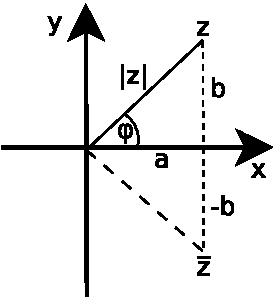
\includegraphics{matematika/obrazky/01-dia1}
\caption{Komplexní číslo ve 2D}
\label{fig:ComplexNum2D}
\end{figure}


Každé komplexní číslo z různé od nuly je možné jednoznačně vyjádřit v \textbf{goniometrickém tvaru}. Pokud si v komplexní rovině zvolíme polární souřadnicový systém, vzdálenost čísla $z$ od počátku je právě jeho absolutní hodnota $|z|$ (také nazývaná \textbf{modul}) a orientovaný úhel $\varphi = |\sphericalangle JOZ|$ (\emph{argument}), kde $J$ je bod $J[1,0]$, $O$ je počátkem soustavy a $Z$ je obraz komplexního čísla $a + bi$ se souřadnicemi $Z[a,b]$, platí:
$$z = |z| (\cos \varphi + i\cdot \sin \varphi)$$

Argument $\varphi$ lze vyjádřit ze vztahů: $\cos \varphi = \frac{a}{|z|}$ a $\sin \varphi = \frac{b}{|z|}$

Pro dělení komplexních čísel $z_1 = |z_1|\cdot (\cos\varphi_1 + i\cdot \sin
\varphi_1)$ a $z_2 = |z_2|\cdot (\cos \varphi_2 + i\cdot \sin \varphi_2)$ platí následující rovnice:
$$\frac{z_1}{z_2} = \frac{|z_1|}{|z_2|}\cdot \left[ \cos(\varphi_1 - \varphi_2) + i\cdot \sin(\varphi_1 - \varphi_2) \right]$$

Pro násobení komplexních čísel $z_1$ a $z_2$ z předchozího příkladu slouží vzorec:
$$z_1 \cdot  z_2 = |z_1|\cdot |z_2|\cdot \left[ \cos(\varphi_1 + \varphi_2) + i\cdot \sin(\varphi_1 + \varphi_2) \right]$$

Pro \textbf{n-tou mocninu komplexní čísla} v goniometrickém tvaru platí tzv. \textbf{Moivreova věta}:
$$z^n = |z|^n (\cos n \varphi + i\cdot \sin n \varphi)$$

\subsection{Posloupnosti a limity}
\begin{definiceN}{posloupnost}
\emph{Posloupností reálných čísel} nazýváme jakékoli zobrazení z množiny $\mathbb{N}$ do množiny $\mathbb{R}$. Posloupnost obvykle značíme symbolem $\{a_n\}^{\infty}_{n=1}$ nebo $\{a_n\}_{n \in \mathbb{N}}$. Pro každé konkrétní $n \in \mathbb{N}$ nazýváme reálné číslo $a_n$ \emph{n-tým členem} posloupnosti $\{a_n\}$.
\end{definiceN}

\begin{definiceN}{Omezené posloupnosti}
\begin{penumerate}
	\item Posloupnost $\{a_n\}$ je \emph{shora omezená}, je-li $\{a_n; n \in \mathbb{N}\}$ shora omezená.
	\item Posloupnost $\{a_n\}$ je \emph{zdola omezená}, je-li $\{a_n; n \in \mathbb{N}\}$ zdola omezená.
	\item Posloupnost $\{a_n\}$ je \emph{omezená}, je-li zdola omezená a shora omezená.
\end{penumerate}
\end{definiceN}

\begin{definiceN}{Rostoucí a klesající posloupnosti}
\begin{penumerate}
	\item Posloupnost $\{a_n\}$ je \emph{klesající}, jestliže $\forall n \in \mathbb{N}: a_n > a_{n+1}$.
	\item Posloupnost $\{a_n\}$ je \emph{rostoucí}, jestliže $\forall n \in \mathbb{N}: a_n < a_{n+1}$.
	\item Posloupnost $\{a_n\}$ je \emph{neklesající}, jestliže $\forall n \in \mathbb{N}: a_n \le a_{n+1}$.
	\item Posloupnost $\{a_n\}$ je \emph{nerostoucí}, jestliže $\forall n \in \mathbb{N}: a_n \ge a_{n+1}$.
	\item Posloupnost $\{a_n\}$ je \emph{monotónní}, jestliže je nerostoucí nebo neklesající.
	\item Posloupnost $\{a_n\}$ je \emph{ryze monotónní}, jestliže je rostoucí nebo klesající.
\end{penumerate}
\end{definiceN}

\subsubsection{Vlastní limity}
\begin{definice}
Nechť $\{a_n\}$ je posloupnost reálných čísel a $A \in \mathbb{R}$. Řekneme, že A je \emph{vlastní limitou posloupnosti} $\{a_n\}$, jestliže
$$\forall \varepsilon > 0\ \exists n_0 \in \mathbb{N}: \forall n \ge n_0, n \in \mathbb{N}: |a_n - A| < \varepsilon$$
značíme
$$\lim_{n \rightarrow \infty} a_n = A$$
\noindent Dá se jednoduše ukázat, že toto je splněno i pokud máme vždy od $n_0$ dále zaručeno jen to, že $|a_n - A| < K\cdot\varepsilon$ pro nějaké $K>0$.
\end{definice}

\begin{definice}
Jestliže existuje $A \in \mathbb{R}$ tak, že $\lim_{n \rightarrow \infty}a_n = A$, pak říkáme, že posloupnost $\{a_n\}$ má \emph{vlastní limitu} nebo že \emph{konverguje} (je \emph{konvergentní}). V opačném případě říkáme, že posloupnost \emph{diverguje}.
\end{definice}

\begin{pozorovani}
Ne každá posloupnost je konvergentní. Například posloupnost 0,1,0,1,0,... nemá vlastní limitu a podobně posloupnost $\{2^n\}$ nemá vlastní limitu.
\end{pozorovani}

\begin{priklady}
\begin{pitemize}
	\item $\lim_{n \rightarrow \infty} (\sqrt{n+1} - \sqrt{n}) = 0$
	\item $\lim_{n \rightarrow \infty} \sqrt[n]{n} = 1$
\end{pitemize}
\end{priklady}

\begin{vetaN}{o jednoznačnosti limity posloupnosti}
Každá posloupnost má nejvýše jednu limitu.
\end{vetaN}

\begin{vetaN}{o omezenosti konvergentní posloupnosti}
Každá konvergentní posloupnost je omezená.
\end{vetaN}

\begin{definice}
Nechť $\{a_n\}_{n \in \mathbb{N}}$ je posloupnost reálných čísel. Řekneme, že posloupnost $\{b_k\}_{k \in \mathbb{N}}$ je \emph{vybraná} z posloupnosti, neboli že posloupnost $\{b_k\}_{k \in \mathbb{N}}$ je \emph{podposloupností} posloupnosti $\{a_n\}_{n \in \mathbb{N}}$, jestliže existuje rostoucí posloupnost přirozených čísel $\{n_k\}$ taková, že $b_k = a_{n_k}$ pro všechna $k \in \mathbb{N}$.
\end{definice}

\begin{vetaN}{o limitě vybrané posloupnosti}
Nechť $\{a_n\}_{n \in \mathbb{N}}$ je posloupnost reálných čísel a nechť $\lim_{n \rightarrow \infty} a_n = A$. Nechť posloupnost $\{b_k\}_{k \in \mathbb{N}}$ je vybraná z posloupnosti $\{a_n\}_{n \in \mathbb{N}}$. Pak $\lim_{k \rightarrow \infty} b_k = A$.
\end{vetaN}

\begin{vetaN}{o aritmetice limit}
Nechť $\{a_n\}_{n \in \mathbb{N}}$ a $\{b_n\}_{n \in \mathbb{N}}$ jsou dvě posloupnosti reálných čísel a nechť $\lim_{n \rightarrow \infty} a_n = A \in \mathbb{R}$ a $\lim_{n \rightarrow \infty} b_n = B \in \mathbb{R}$. Pak platí:
\begin{penumerate}
	\item $\lim_{n \rightarrow \infty} (a_n+b_n) = A+B$
	\item $\lim_{n \rightarrow \infty} (a_n \cdot  b_n) = A\cdot B$
	\item je-li $\forall n \in \mathbb{N}: b_n \neq 0$ a $B \neq 0$, pak $\lim_{n \rightarrow \infty} \frac{a_n}{b_n}=\frac{A}{B}$
\end{penumerate}
\end{vetaN}

\begin{vetaN}{o limitě a uspořádání}
Nechť $\{a_n\}_{n \in \mathbb{N}}$ a $\{b_n\}_{n \in \mathbb{N}}$ jsou dvě posloupnosti reálných čísel a nechť $\lim_{n \rightarrow \infty} a_n = A \in \mathbb{R}$ a $\lim_{n \rightarrow \infty} b_n = B \in \mathbb{R}$. Pak platí:
\begin{penumerate}
	\item Jestliže $A < B$, potom $\exists n_0 \in \mathbb{N}\ \forall n > n_0: a_n < b_n$
	\item Jestliže $\exists n_0 \in \mathbb{N}\ \forall n \ge n_0: a_n \ge b_n$, pak $A \ge B$
\end{penumerate}

\noindent Pozor, ostrost nerovností v tomto případě je důležitá.
\end{vetaN}

\begin{vetaN}{o policajtech}
Nechť $\{a_n\}_{n \in \mathbb{N}}$, $\{b_n\}_{n \in \mathbb{N}}$ a $\{c_n\}_{n \in \mathbb{N}}$ jsou posloupnosti reálných čísel, splňující
\begin{penumerate}
	\item $\exists n_0 \in \mathbb{N}\ \forall n > n_0: a_n \le c_n \le b_n$
	\item $\lim_{n \rightarrow \infty}a_n = \lim b_n = A \in \mathbb{R}$
\end{penumerate}
Pak
$$
\lim c_n = A
$$
\end{vetaN}

\begin{vetaN}{o limitě součinu mizející ($\lim=0$) a omezené posloupnosti}
Nechť $\{a_n\}_{n \in \mathbb{N}}$ a $\{b_n\}_{n \in \mathbb{N}}$ jsou posloupnosti reálných čísel, nechť je $\lim_{n \rightarrow \infty} a_n = 0$ a $\{b_n\}$ omezená. Pak
$$
\lim_{n \rightarrow \infty}(a_n \cdot b_n) = 0
$$
\end{vetaN}

\subsubsection{Nevlastní limity}
\begin{definice}
Řekneme, že posloupnost  $\{a_n\}$ má \emph{nevlastní limitu} $+ \infty$, jestliže:
$$ \forall K \in \mathbb{R}\ \exists n_0 \in \mathbb{N}: \forall n \ge n_0, n \in \mathbb{N}: a_n \ge K $$

Obdobně řekneme, že posloupnost  $\{a_n\}$ má \emph{nevlastní limitu} $- \infty$, jestliže:
$$ \forall K \in \mathbb{R}\ \exists n_0 \in \mathbb{N}: \forall n \ge n_0, n \in \mathbb{N}: a_n \le K $$

Má-li posloupnost nevlastní limitu, říkáme o ní, že diverguje, stejně jako v případě, že žádnou limitu nemá.
\end{definice}

\begin{poznamka}
Všechny možné situace jsou znázorněny na následujícím diagramu:

limita posloupnosti:
\begin{pitemize}
	\item neexistuje
	\item existuje
	\begin{pitemize}
		\item vlastní
		\item nevlastní
		\begin{pitemize}
			\item $- \infty$
			\item $+ \infty$
		\end{pitemize}
	\end{pitemize}
\end{pitemize}

\end{poznamka}

\begin{definice}
Množinu $\mathbb{R}^* := \mathbb{R} \cup \{ + \infty, - \infty \}$ nazýváme \emph{rozšířenou reálnou osou}.
\end{definice}

\begin{poznamka}
Věty o jednoznačnosti limity, o limitě vybrané posloupnosti, o limitě a uspořádání a o policajtech platí v nezměněné podobě, jestliže připustíme nevlastní limity. Věta o omezenosti konvergentní posloupnosti zrejmě neplatí - neboť je-li $\lim_{n \rightarrow \infty} a_n=\infty$ (nebo $- \infty$), pak posloupnost $\{a_n\}$ není omezená. Větu o aritmetice limit pro rozšírenou osu uvedeme zvlášť.
\end{poznamka}

\begin{vetaN}{o aritmetice limit pro nevlastní limity}
Nechť $\{a_n\}_{n \in \mathbb{N}}$ a $\{b_n\}_{n \in \mathbb{N}}$ jsou dvě posloupnosti reálných čísel a nechť $\lim_{n \rightarrow \infty} a_n = A \in \mathbb{R}^*$ a $\lim_{n \rightarrow \infty} b_n = B \in \mathbb{R}^*$. Pak platí:
\begin{penumerate}
	\item $\lim_{n \rightarrow \infty} (a_n+b_n) = A+B \textit{, pokud je výraz A+B definován}$
	\item $\lim_{n \rightarrow \infty} (a_n \cdot  b_n) = A\cdot B\textit{, pokud je výraz }A\cdot B\textit{ definován}$
	\item je-li $\forall n \in \mathbb{N}: b_n \neq 0$ a $B \neq 0$, pak $\lim_{n \rightarrow \infty} \frac{a_n}{b_n}=\frac{A}{B} \textit{, pokud je výraz } \frac{A}{B} \textit{ definován}$
\end{penumerate}
\end{vetaN}

\begin{definiceN}{Supremum a infimum na rozšířené reálné ose}
\begin{pitemize}
	\item Nechť množina $A \subset \mathbb{R}$ je shora neomezená. Pak klademe $\sup A := +\infty$
	\item Nechť množina $A \subset \mathbb{R}$ je zdola neomezená. Pak klademe $\inf A := -\infty$
	\item Nechť $A=\emptyset$. Pak klademe $\sup A := -\infty$ a $inf A := +\infty$
\end{pitemize}
\end{definiceN}

\begin{poznamka}
Prázdná množina je jediná množina, jejíž supremum je menší než její infimum.
\end{poznamka}

\begin{vetaN}{o limitě podílu kladné a mizející posloupnosti}
Nechť $\{a_n\}_{n \in \mathbb{N}}$ a $\{b_n\}_{n \in \mathbb{N}}$ jsou posloupnosti reálných čísel, nechť je $\lim_{n \rightarrow \infty} a_n = A \in \mathbb{R}^*, A>0$ a nechť $\lim_{n \rightarrow \infty}\{b_n\}=0$. Nechť
$$
	\exists n_0 \in \mathbb{N} \textit{ } \forall n \ge n_0, n \in \mathbb{N}: b_n>0
$$
Pak
$$
	\lim_{n \rightarrow \infty} \frac{a_n}{b_n} = + \infty
$$
\end{vetaN}

\subsubsection{Monotónní posloupnosti}
\begin{vetaN}{o limitě monotónní posloupnosti}
Každá monotónní posloupnost má limitu.
\end{vetaN}

\begin{poznamka}
Je-li posloupnost neklesající (nerostoucí) a navíc shora (zdola) omezená, pak má vlastní limitu.
Je-li posloupnost neklesající (nerostoucí) a navíc shora (zdola) neomezená, pak má limitu $+ \infty$ ($- \infty$).
\end{poznamka}

\begin{definiceN}{Limes superior a limes inferior}
Nechť $\{a_n\}_{n \in \mathbb{N}}$ je posloupnost reálných čísel. Je-li $\{a_n\}$ shora omezená, definujeme posloupnost $\{b_n\}_{n \in \mathbb{N}}$ předpisem:
$$
	b_n := \sup\{a_k; k \ge n \}
$$
Je-li $\{a_n\}$ zdola omezená, definujeme posloupnost $\{c_n\}_{n \in \mathbb{N}}$ předpisem:
$$
	c_n := \inf\{a_k; k \ge n \}
$$
V takovém případě definujeme:
$$
\lim \sup~a_n := \left\{
\begin{array}{ll} \lim_{n \rightarrow \infty} b_n & \textit{jestliže je } \{a_n\} \textit{ shora omezená} \\ \infty & \textit{jestliže je } \{a_n\} \textit{ shora neomezená} \end{array}
\right.
$$
Tuto hodnotu nazýváme \emph{limes superior} posloupnosti $\{a_n\}_{n \in \mathbb{N}}$. Obdobně definujeme \emph{limes inferior} posloupnosti $\{a_n\}_{n \in \mathbb{N}}$ předpisem:
$$
\lim \inf~a_n := \left\{
\begin{array}{ll} \lim_{n \rightarrow \infty} c_n & \textit{jestliže je } \{a_n\} \textit{ zdola omezená} \\ - \infty & \textit{jestliže je } \{a_n\} \textit{ zdola neomezená} \end{array}
\right.
$$
\end{definiceN}

\begin{poznamka}
Limes superior a limes inferior jsou vždy dobře definované hodnoty a platí
$$
\lim \sup~a_n \in \mathbb{R}^*, \lim \inf~a_n \in \mathbb{R}^*, 
$$
Na rozdíl od limity, která nemusí existovat, tyto dvě hodnoty existují pro
libovolnou posloupnost reálných čísel.
\end{poznamka}

\begin{vetaN}{o vztahu limity, limes superior a limes inferior}
Nechť $\{a_n\}_{n \in \mathbb{N}}$ je posloupnost reálných čísel. Potom 
$$
	\lim a_n = A \in \mathbb{R}^{*}
$$
právě tehdy, když
$$
\lim \sup~a_n = \lim \inf~a_n = A \in \mathbb{R}^*
$$
\end{vetaN}

\begin{definice}
Nechť $\{a_n\}_{n \in \mathbb{N}}$ je posloupnost reálných čísel. Pak $A \in \mathbb{R}^*$ nazveme \emph{hromadnou hodnotou} posloupnosti $\{a_n\}$, jestliže existuje vybraná posloupnost taková $\{a_{n_k}\}$, že $\lim_{k \rightarrow \infty} a_{n_k} = A$. Množina všech hromadných hodnot značíme $H(\{a_n\})$
\end{definice}

\begin{vetaN}{o vztahu limes superior, limes inferior a hromadných hodnot}
Nechť $\{a_n\}_{n \in \mathbb{N}}$ je posloupnost reálných čísel. Potom $H\{(a_n)\} \neq \emptyset$,
$$
\lim \sup~a_n = \max H(\{a_n\}) \textit{ a } \lim \inf~a_n = \min H(\{a_n\})
$$
\end{vetaN}

\subsection{Cauchyovské posloupnosti}

Tato sekce je vypracovaná podle skript Prof. A. Pultra z matematické analýzy\\
(\texttt{http://kam.mff.cuni.cz/\~{}pultr/})
\bigskip

\begin{definiceN}{Bolzano-Cauchyova podmínka}
Řekneme, že posloupnost $\{a_n\}_{n\geq 0}$ je \emph{cauchyovská}, nebo-li že splňuje \emph{Bolzano-Cauchyho podmínku}, pokud pro ní platí:
$$
\forall \varepsilon > 0~~\exists n_0 \in \mathbb{N}: \forall m, n \in \mathbb{N}: m \ge n_0, n \ge n_0: |a_n - a_m| < \varepsilon
$$
\end{definiceN}

\begin{vetaN}{Bolzano-Weierstrassova}
Z každé omezené posloupnosti lze vybrat konvergentní podposloupnost. Jsou-li $a_n$ v kompaktním intervalu $[a,b]$, je limita vybrané posloupnosti v tomto intervalu.

\medskip\begin{dukaz}
První část dokážeme nalezením takové posloupnosti. Vezmeme $A:=\lim\sup~a_n$ a definujeme pro každé $k\in\mathbb{N}$ množinu $M_k:=\{j\in\mathbb{N}|j>n_{k-1},a_j\in\langle A - \frac{1}{2^k}, A + \frac{1}{2^k}\rangle\}$ a $n_k:=\min M_k$. Potom $\{a_{n_k}\}$ je vybraná posloupnost, která konverguje. Druhá část je přímým důsledkem věty o limitě a uspořádání.
\end{dukaz}
\end{vetaN}

\begin{lemma}
Má-li cauchyovská posloupnost konvergentní podposloupnost, je konvergentní.

\medskip\begin{dukaz}
Nechť $\lim a_{n_k} = x$. Pro $\varepsilon > 0$ zvolme $n_0$, aby pro $m,n\geq n_0$ platilo $|a_m-a_n|<\frac{\varepsilon}{2}$ a $|a_k-x|<\frac{\varepsilon}{2}$. Protože $k_n\geq n$, platí $|a_n-x|=|a_n-a_{k_n}|+|a_{k_n}-x|<\varepsilon$.
\end{dukaz}
\end{lemma}


\begin{vetaN}{Bolzano-Cauchyova}
Posloupnost $\{a_n\}$ má vlastní limitu, právě když je cauchyovská.

\medskip\begin{dukaz}
\begin{penumerate}
    \item Implikace \uv{$\Rightarrow$} je hned vidět -- stačí vzít k $\varepsilon$ takové $n_0$, že $|a_n-x|<\frac{\varepsilon}{2}\ \forall n\geq n_0$. Potom je $|a_n-a_m|=|a_n-x+x-a_m|\leq|a_n-x|+|x-a_m|\leq\varepsilon\ \forall m,n\geq n_0$.\medskip
    \item Pro druhou implikaci stačí dokázat, že je cauchyovská posloupnost omezená a zbytek dostaneme z předchozího lemmatu a Bolzano-Weierstrassovy věty. Pro $\varepsilon=1$ existuje $n_0$ takové, že $a_{n_0}-1<a_n<a_{n_0}+1$ pro každé $n\geq n_0$ (to plyne přímo z podmínky), takže zbývá jen konečný počet členů mimo toto rozmezí (pro $n<n_0$), a ty vždy tvoří omezený systém.
\end{penumerate}
\end{dukaz}
\end{vetaN}

